% Compile with XeLaTeX !!
\documentclass[12pt,a4paper]{article}

% -------------------------------------------------
% Fonts & Greek language via polyglossia
% -------------------------------------------------
\usepackage{fontspec}
\usepackage{polyglossia}

\setmainlanguage{greek}
\setotherlanguage{english}

% Choose fonts (any system font works)
\setmainfont{Times New Roman}
\setsansfont{Arial}
\setmonofont{Courier New}

% -------------------------------------------------
% Math & Graphics
% -------------------------------------------------
\usepackage{amsmath, amssymb, amsfonts}
\usepackage{graphicx}
\usepackage{float}
\usepackage{geometry}
\usepackage{caption}
\usepackage{subcaption}
\usepackage{hyperref}

\geometry{margin=2.5cm}

\title{\textbf{Τεχνικές Βελτιστοποίησης}\\
	\large Εργασία 1}
\author{Πελοπίδας-Νικόλαος Τσιούντσιουρας \\ ΑΕΜ: 11085}
\date{\today}

\begin{document}
	
	\maketitle
	\tableofcontents
	\newpage
	
	\section{Εισαγωγή}
	
	Ζητούμενο της εργασίας είναι η ελαχιστοποίηση μίας δοσμένης κυρτής συνάρτησης $f(x)$ όταν $x \in [a, b]$. Το πρόβλημα αυτό αποτελεί τη βάση των αλγορίθμων εύρεσης ελαχίστου συναρτήσεων με περισσότερες μεταβλητές. Οι αλγόριθμοι που θα υλοποιηθούν είναι:
	\begin{enumerate}
		\item Μέθοδοι αναζήτησης ελαχίστου χωρίς χρήση παραγώγων:
		\begin{itemize}
			\item Μέθοδος της Διχοτόμου,
			\item Μέθοδος του Χρυσού Τομέα,
			\item Μέθοδος Fibonacci.
		\end{itemize}
		\item Μέθοδοι αναζήτησης με χρήση παραγώγων:
		\begin{itemize}
			\item Μέθοδος της Διχοτόμου με χρήση παραγώγου.
		\end{itemize}
	\end{enumerate}
	
	Σε όλες τις παραπάνω μεθόδους ξεκινάμε από ένα αρχικό διάστημα $[a, b]$ μέσα στο οποίο βρίσκεται το ελάχιστο $x^{*}$ της $f(x)$. Με τη χρήση ενός ακολουθιακού αλγορίθμου καταλήγουμε σε ένα διάστημα $[a_{k}, b_{k}]$ με προδιαγεγραμμένη ακρίβεια $l>0$, δηλαδή $b_{k}-a_{k} \le l$. 
	
	Στη συγκεκριμένη περίπτωση, το αρχικό διάστημα $[a, b]$ είναι το $[-1, 3]$, ενώ οι συναρτήσεις που θα ελαχιστοποιηθούν είναι:
	\begin{itemize}
		\item $f_{1}(x)=5^{x}+(2-\cos\left(x\right))^{2}$
		\item $f_{2}(x)=(x-1)^{2}+e^{x-5}\sin\left(x+3\right)$
		\item $f_{3}(x)=e^{-3x}-(\sin\left(x-2\right)-2)^{2}$
	\end{itemize}	
	
	Για τις παραπάνω μεθόδους και συναρτήσεις θα μελετηθεί ο αριθμός των υπολογισμών της $f$ συναρτήσει του τελικού εύρους αναζήτησης $l$, καθώς και το πώς μεταβάλλεται το διάστημα $[a_{k}, b_{k}]$ συναρτήσει του δείκτη επαναλήψεων k για διάφορες τιμές του τελικού εύρους αναζήτησης $l$. Επίσης, για τη μέθοδο της διχοτόμου χωρίς χρήση παραγώγων θα μελετηθεί και ο αριθμός των υπολογισμών της $f$ συναρτήσει της σταθεράς $\epsilon$.
	
	\section{Θεωρία}
	Όλες οι μέθοδοι που θα υλοποιηθούν και θα εξεταστούν βασίζονται στο Θεώρημα 5.1.1. Επίσης, μας δίνεται ότι οι δοθείσες συναρτήσεις είναι κυρτές, επομένως δεν χρειάζεται στη συγκεκριμένη περίπτωση έλεγχος για την κυρτότητα των συναρτήσεων.
	
	\subsection{Μέθοδος Διχοτόμου}
	Στη μέθοδο της \textbf{Διχοτόμου} επιλέγουμε δύο σημεία που απέχουν $\epsilon$ από το μέσο του διαστήματος $[a_k, b_k]$, υπολογίζουμε τις τιμές της $f$ στο σημείο αυτό και μετά με βάση τις τιμές αυτές επιλέγουμε το νέο διάστημα αναζήτησης. Συνεχίζουμε να επαναλαμβάνουμε τη διαδικασία αυτή μέχρις ότου το εύρος του διαστήματος $[a_k, b_k]$ να γίνει μικρότερο του $l$. Δηλαδή, ο αλγόριθμος συνοπτικά είναι ο εξής:
	\begin{itemize}
		\item Θέτω:
		\[x_{1k} = \dfrac{a_k+b_k}{2} - \epsilon , x_{2k} = \dfrac{a_k+b_k}{2} +- \epsilon\]
		\item Αν $f(x_{1k})<f(x_{2k})$, θέτω $a_{k+1}=a_k$ και $b_{k+1}=x_{2k}$. Διαφορετικά, θέτω $a_{k+1}=x_{1k}$ και $b_{k+1}=b_k$. Θέτω μετά $k=k+1$ και συνεχίζω μέχρις ότου $b_k-a_k<l$.
	\end{itemize}
	Ενώ είναι αρκετά εύκολη στην υλοποίησή της και δεν απαιτεί καμία ιδιαίτερη γνώση για τη συνάρτηση, χρειάζεται αρκετούς υπολογισμούς της $f$ (δύο υπολογισμοί σε κάθε επανάληψη).
	
	\subsection{Μέθοδος Χρυσού Τομέα}
	Η μέθοδος του \textbf{Χρυσού Τομέα} τοποθετεί τα σημεία αναζήτησης με σταθερό τρόπο. Σε κάθε βήμα το διάστημα $[a_{k}, b_{k}]$ συρρικνώνεται με σταθερή αναλογία, ενώ χρειάζεται μόνο ένας υπολογισμός της $f$, γιατί το ένα από τα δύο σημεία ανακυκλώνεται. Επίσης, το εύρος του νέου υποδιαστήματος συνδέεται με το προηγούμενο με μία σταθερά αναλογίας $\gamma$. Συνοπτικά ο αλγόριθμος δίνεται ως εξής:
	\begin{itemize}
		\item Θέτω:
		\[x_{1k} = a_k + (1-\gamma)(b_k-a_k) , x_{2k} = a_k + \gamma(b_k-a_k)\] όπου $\gamma=0.618$.
		\item Αν $f(x_{1k})<f(x_{2k})$, θέτω $a_{k+1}=a_k$ και $b_{k+1}=x_{2k}$. Επιπλέον, $x_{2k+1}=x_{1k}$ και $x_{1k+1} = a_{k+1} + \gamma(b_{k+1}-a_{k+1})$, υπολογίζω την $f(x_{1k+1})$ και θέτω $k=k+1$.
		\item Αν $f(x_{1k})>f(x_{2k})$, θέτω $a_{k+1}=x_{1k}$ και $b_{k+1}=b_k$. Επιπλέον, $x_{1k+1}=x_{2k}$ και $x_{2k+1} = a_{k+1} + (1-\gamma)(b_{k+1}-a_{k+1})$, υπολογίζω την $f(x_{2k+1})$ και θέτω $k=k+1$.
		\item Συνεχίζω έτσι έως ότου $b_k-a_k<l$. 
	\end{itemize}
	Βλέπυμε ότι στη συγκεκριμένη μέθοδο πέρα από την αρχική επανάληψη στην οποία απαιτούνται δύο υπολογισμοί της $f$, σε όλες τις υπόλοιπες χρειάζεται μόνο ένας, αφού το ένα σημείο ανακυκλώνεται.
	
	\subsection{Μέθοδος Fibonacci}
	Η μέθοδος \textbf{Fibonacci} μοιάζει με τη μέθοδο του Χρυσού Τομέα, αλλά διαφοροποιείται στο ότι το υποδιάστημα αναζήτησης στην $k$ επανάληψη δεν συνδέεται με αυτό της $k-1$ με μία σταθερά αλλά μεταβάλλεται από επανάληψη σε επανάληψη. Για τον ορισμό των σημείων $x_{1k}, x_{2k}$ χρησιμοποιείται η ακολουθία \textit{Fibonacci}.Συνοπτικά ο αλγόριθμος δίνεται ως εξής:
	\begin{itemize}
		\item Υπολογίζω τον συνολικό αριθμό των υπολογισμών $n$ της $f$ έτσι ώστε: $F_n>\dfrac{b_1-a_1}{l}$, όπου $F_n$ η ακολουθία Fibonacci.
		\item Θέτω:
		\[x_{1k} = a_k + \dfrac{F_{N-k-1}}{F_{N-k+1}}(b_k-a_k) , x_{2k} = a_k + \dfrac{F_{N-k}}{F_{N-k+1}}(b_k-a_k)\].
		\item Αν $f(x_{1k})<f(x_{2k})$, θέτω $a_{k+1}=a_k$ και $b_{k+1}=x_{2k}$. Επιπλέον, $x_{2k+1}=x_{1k}$ και $x_{1k+1} = a_{k+1} + \dfrac{F_{N-k-2}}{F_{N-k}}(b_{k+1}-a_{k+1})$. Αν $k\ne n-2$, υπολογίζω την $f(x_{1k+1})$ και θέτω $k=k+1$.
		\item Αν $f(x_{1k})>f(x_{2k})$, θέτω $a_{k+1}=x_{1k}$ και $b_{k+1}=b_k$. Επιπλέον, $x_{1k+1}=x_{2k}$ και $x_{2k+1} = a_{k+1} + \dfrac{F_{N-k-1}}{F_{N-k}}(b_{k+1}-a_{k+1})$. Αν $k\ne n-2$, υπολογίζω την $f(x_{2k+1})$ και θέτω $k=k+1$.
		\item Αν $k=n-2$, θέτω $x_{1n}=x_{1n-1}$ και $x_{2n}=x_{1n-1}+\epsilon$, όπου $\epsilon$ μία σταθερά. Αν $f(x_{1n})>f(x_{2n})$, θέτω $a_n=x_{1n}$ και $b_n=b_{n-1}$. Διαφπρετικά θέτω $a_n=a_{n-1}$ και $b_n=x_{2n}$ και ο αλγόριθμος τερματίζει.
	\end{itemize}
	Όπως και στη μέθοδο του Χρυσού Τομέα, πέραν την αρχικής επανάληψης σε όλες τις υπόλοιπες απαιτείται μόνον ένας υπολογισμός της συνάρτησης. Ωστόσο, πρέπει να υπολογίσουμε εκ των προτέρων τις επαναλήψεις του αλγορίθμου.
	
	\subsection{Μέθοδος Διχοτόμου Με Χρήση Παραγώγων}
	Η μέθοδος της \textbf{Διχοτόμου με χρήση Παραγώγων} αξιοποιεί την πληροφορία της πρώτης παραγώγου της συνάρτησης $f$ για να εντοπίσει σε ποιά κατεύθυνση βρίσκεται το ελάχιστο. Σε κάθε βήμα επιλέγεται το μέσο σημείο και υπολογίζεται η πρώτη παράγωγους της $f$ στο σημείο αυτό. Αν η παράγωγος είναι θετική, το ελάχιστο βρίσκεται αριστερά, ενώ αν είναι αρνητική, το ελάχιστο βρίσκεται στα δεξιά. Σε περίπτωση που η παράγωγος μηδενιστεί, ο αλγόριθμος έχει εντοπίσει το σημείο στο οποίο η συνάρτηση ελαχιστοποιείται και σταματά. Συνοπτικά ο αλγόριθμος δίνεται ως εξής:
	\begin{itemize}
		\item Υπολογίζω τον συνολικό αριθμό των υπολογισμών $n$ της $f$ έτσι ώστε: $(\dfrac{1}{2})^n \leq \dfrac{l}{b_1-a_1}$.
		\item Θέτω:
		\[x_k = \dfrac{a_k+b_k}{2}\] και υπολογίζω $\left. \frac{df(x)}{dx} \right|_{x = x_k}$.
		\item Αν $\left. \frac{df(x)}{dx} \right|_{x = x_k}>0$, θέτω $a_{k+1}=a_k$ και $b_{k+1}=x_{k}$.
		\item Αν $\left. \frac{df(x)}{dx} \right|_{x = x_k}<0$, θέτω $a_{k+1}=x_{k}$ και $b_{k+1}=b_k$.
		\item Αν $k=n$ ή $\left. \frac{df(x)}{dx} \right|_{x = x_k}=0$, ο αλγόριθμος τερματίζει. Διαφορετικά, θέτω $k=k+1$ και επαναλαμβάνω τη διαδικασία.
	\end{itemize}
	Η μέθοδος αυτή αξιοποιεί την παράγωγο της $f$ και για αυτό συγκλίνει πιο γρήγορα. Ωστόσο, είναι απαραίτητο η συνάρτηση να είναι παραγωγίσιμη.
	
	\section{Πειράματα}
	
	Το διάστημα αναζήτησης ήταν $[-1, 3]$ και εξετάστηκαν οι συναρτήσεις:
	
	\[
	f_1(x) = 5^x + (2 - \cos x)^2
	\]
	
	\[
	f_2(x) = (x-1)^2 + e^{x-5}\sin(x+3)
	\]
	
	\[
	f_3(x) = e^{-3x} - (\sin(x-2)-2)^2
	\]
	
	\subsection{Μέθοδος Διχοτόμου}
	
	\subsubsection{Μεταβολή υπολογισμών της $f$ συναρτήσει του $\epsilon$}
	
	Στο πρώτο πείραμα εξετάζεται η μεταβολή του αριθμού υπολογισμών της $f$ συναρτήσει της σταθεράς $ε$. Παρατηρούμε ότι και στις τρεις συναρτήσεις παρατηρείται η ίδια συμπεριφορά: όσο μικραίνει το $\epsilon$, τόσο αυξάνεται ο αριθμός υπολογισμών της συνάρτησης (δηλαδή αυξάνεται ο αριθμός επαναλήψεων που απαιτούνται για να εκτελεστεί η μέθοδος). Τα γραφήματα έχουν χαρακτηριστική "σκαλωτή" μορφή, επειδή ο τύπος για το πλήθος των επαναλήψεων στη μέθοδο της διχοτόμου δίνει πάντα ακέραιο αριθμό, που αυξάνεται απότομα κάθε φορά που περνάμε σε μικρότερο $\epsilon$. Στο συγκεκριμένο πείραμα το $\epsilon$ παίρνει τιμές από 0.001 έως 0.005 (100 διαφορετικές τιμές που ισαπέχουν μεταξύ τους). Και στις τρεις περιπτώσεις η αύξηση είναι σχεδόν ταυτόσημη, κάτι ανμενόμενο, αφού η μέθοδος της διχοτόμου εξαρτάται κυρίως από το μήκος του διαστήμαοτς και όχι από τη μορφή της συνάρτησης. Άρα, το συμπέρασμα είναι το εξής: ο αριθμός των υπολογισμών της $f$ αυξάνει λογαριθμικά με το $1/ε$ και η μέθοδος γίνεται ακριβέστερη αλλά πιο αργή καθώς ζητάμε μεγαλύτερη ακρίβεια.
	Παρακάτω παραθέτω τα τρία γραφήμματα που δείχνουν πώς μεταβάλλεται ο αριθμός των υπολογισμών της $f$ όσο μεταβάλλουμε την σταθερά $ε$.
	\begin{figure}[H]
		\centering
		\includegraphics[width=0.7\textwidth]{dichotomous_e_vs_fevals_f1.png}
		\caption{Μεταβολή υπολογισμών $f_1$ συναρτήσει του $\epsilon$}
	\end{figure}
	
	\begin{figure}[H]
		\centering
		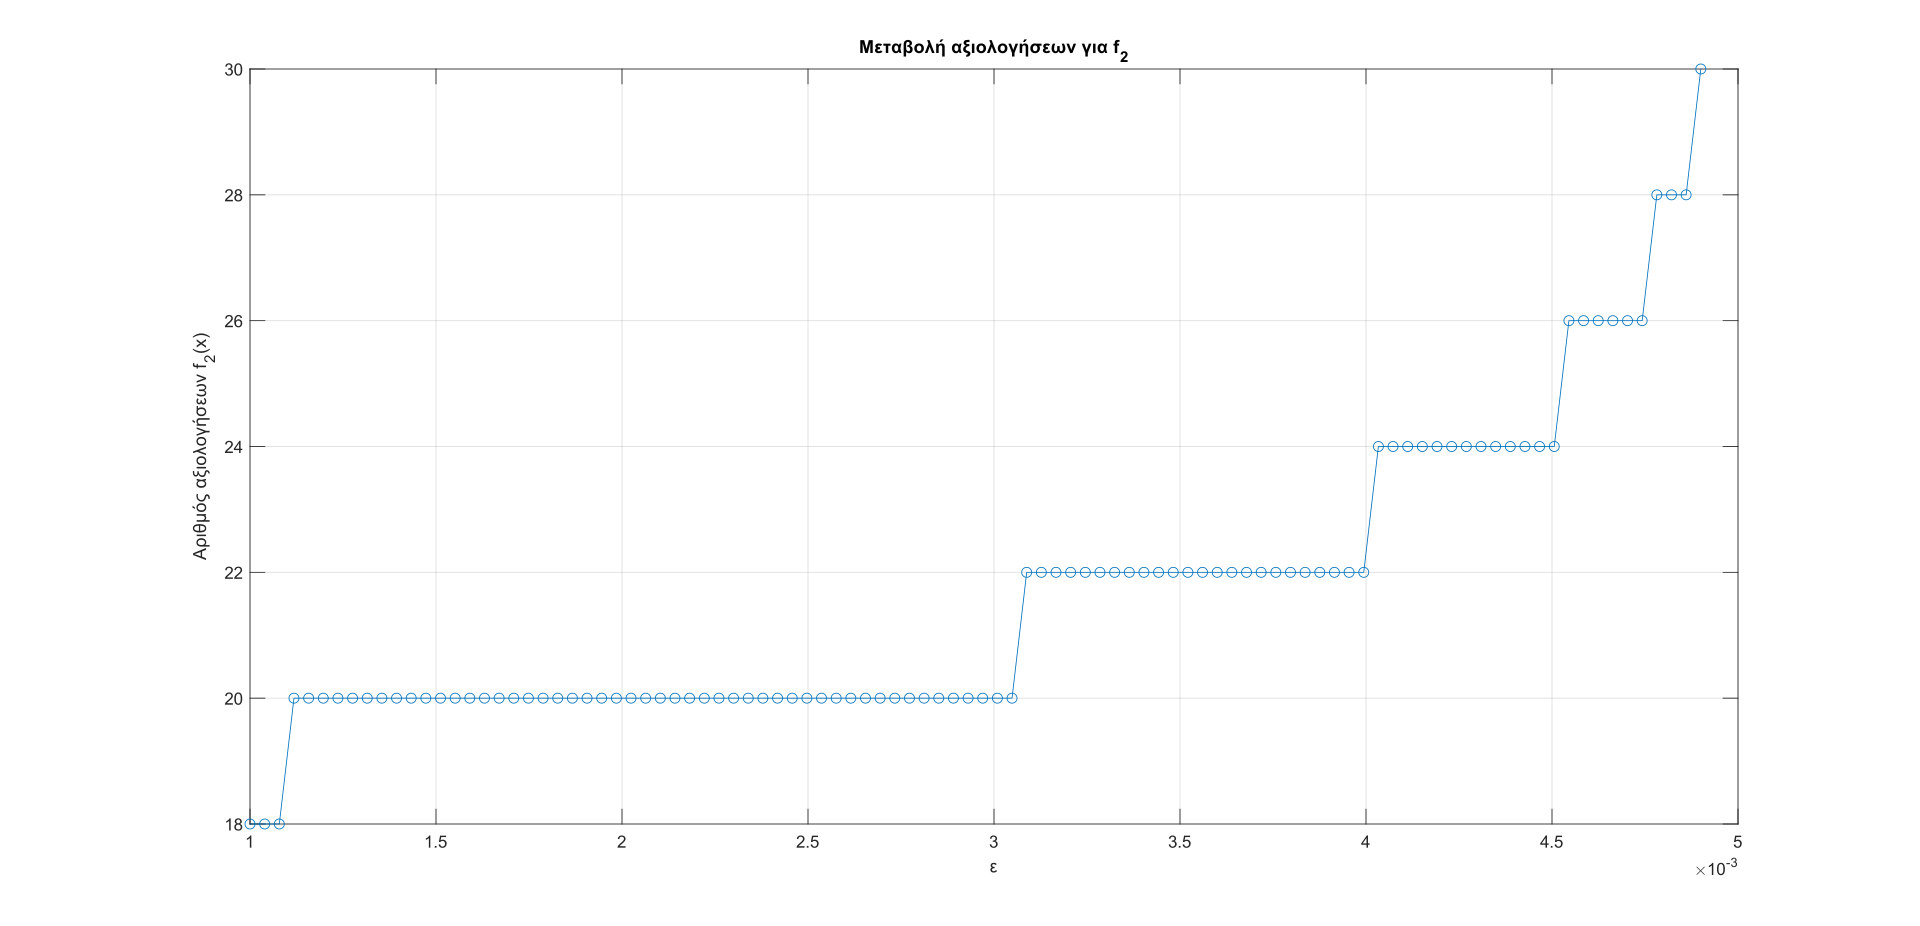
\includegraphics[width=0.7\textwidth]{dichotomous_e_vs_fevals_f2.png}
		\caption{Μεταβολή υπολογισμών $f_2$ συναρτήσει του $\epsilon$}
	\end{figure}
	
	\begin{figure}[H]
		\centering
		\includegraphics[width=0.7\textwidth]{dichotomous_e_vs_fevals_f3.png}
		\caption{Μεταβολή υπολογισμών $f_3$ συναρτήσει του $\epsilon$}
	\end{figure}
	
	
	\subsubsection{Μεταβολή υπολογισμών της $f$ συναρτήσει του $l$}
	Στο δεύτερο πείραμα μεταβάλλω το επιτρεπτό τελικό μήκος διαστήματος $l$ και μετράω πόσες φορές χρειάστηκε να υπολογίσω την $f$ έως ότου η μέθοδος να μειώσει το αρχικό διάστημα στο όριo αυτό. Το αποτέλεσμα είναι το αντίστροφο σε σχέση με το προηγούμενο πείραμα: όσο αυξάνεται το $l$ (δηλαδή όσο λιγότερο απαιτητική γίνεται η ακρίβεια), τόσο μικραίνει ο αριθμός υπολογισμών της $f$. Όπως και στο προηγούμενο πείραμα, έτσι και εδώ εμφανίζεται μία λογαριθμική συμπεριφορά με πολύ ομαλή πτώση. Τα γραφήμματα των τριών συναρτήσεων είναι σχεδόν πανομοιότυπα, επιβεβαιώνοντας ότι η πολυπλοκότητα της μεθόδου είναι γεωμετρική και δεν εξαρτάται ιδιαίτερα από το σχήμα της συνάρτησης. Η ερμηνεία είναι απλή: όσο πιο μεγάλο είναι το τελικό εύρος διαστήματος, τόσο πιο γρήγορα τερματίζει ο αλγόριθμος, άρα χρειάζονται λιγότεροι υπολογισμοί της συνάρτησης.
	Παρακάτω παραθέτω τα τρία γραφήμματα που δείχνουν πώς μεταβάλλεται ο αριθμός των υπολογισμών της $f$ όσο μεταβάλλουμε την σταθερά $l$.
	\begin{figure}[H]
		\centering
		\includegraphics[width=0.7\textwidth]{dichotomous_l_vs_fevals_f1.png}
		\caption{Μεταβολή υπολογισμών $f_1$ συναρτήσει του $l$}
	\end{figure}
	
	\begin{figure}[H]
		\centering
		\includegraphics[width=0.7\textwidth]{dichotomous_l_vs_fevals_f2.png}
		\caption{Μεταβολή υπολογισμών $f_2$ συναρτήσει του $l$}
	\end{figure}
	
	\begin{figure}[H]
		\centering
		\includegraphics[width=0.7\textwidth]{dichotomous_l_vs_fevals_f3.png}
		\caption{Μεταβολή υπολογισμών $f_3$ συναρτήσει του $l$}
	\end{figure}
	
	\subsubsection{Μεταβολή διαστήματος $[a_k,\, b_k]$ συναρτήσει του $k$}
	Στο τρίτο πείραμα εξετάζω πώς συρρικνώνεται το διάστημα αναζήτησης $[a_k, b_k]$ σε κάθε επανάληψη για διάφορες τιμές του $l$. Τα γραφήμματα δείχνουν καθαρά το βασικό χαρακτηριστικό της μεθόδου: το διάστημα μειώνεται με σταθερό ρυθμό κατά $1/2$ κάθε φορά, ανεξάρτητα από τη συνάρτηση. Για μεγάλα $l$, το διάστημα σταθεροποιείται πολύ γρήγορα σε ένα σχετικά τραχύ εύρος τιμών γύρω από το ελάχιστο. Για μικρά $l$, αντίθετα, χρειάζονται πολλές επαναλήψεις και το διάστημα συγκλίνει σταθερά προς τη βέλτιστη τιμή. Εντυπωσιακό είναι ότι στα διαφορετικά $l$ οι καμπύλες "κάθονται" η μία πάνω στην άλλη στα τελευταία βήματα, δείχνοντας ότι η μέθοδος τελικά οδηγεί σε μια πολύ μικρή περιοχή γύρω από το ελάχιστο, ανεξάρτητα από το αρχικό βήμα, αρκεί να επιτρέψουμε αρκετές επαναλήψεις. Επιπλέον, η μορφή του διαστήματος αλλάζει ανάλογα με τη γεωμετρία της συνάρτησης: για τη $f_1$ το διάστημα συγκλίνει κοντά στο −0.35, για τη $f_2$ κοντά στο 1, και για τη $f_3$ κοντά στο 0.5, όπως αναμενόταν από το σχήμα των συναρτήσεων.
	Παρακάτω παραθέτω τα τρία γραφήμματα που δείχνουν πώς μεταβάλλεται το διάστημα $[a_k, b_k]$ συναρτήσει των επαναλήψεων $k$:
	\begin{figure}[H]
		\centering
		\includegraphics[width=0.7\textwidth]{dichotomous_interval_f1.png}
		\caption{Μεταβολή διαστήματος $[a_k, b_k]$ για την $f_1(x)$}
	\end{figure}
	
	\begin{figure}[H]
		\centering
		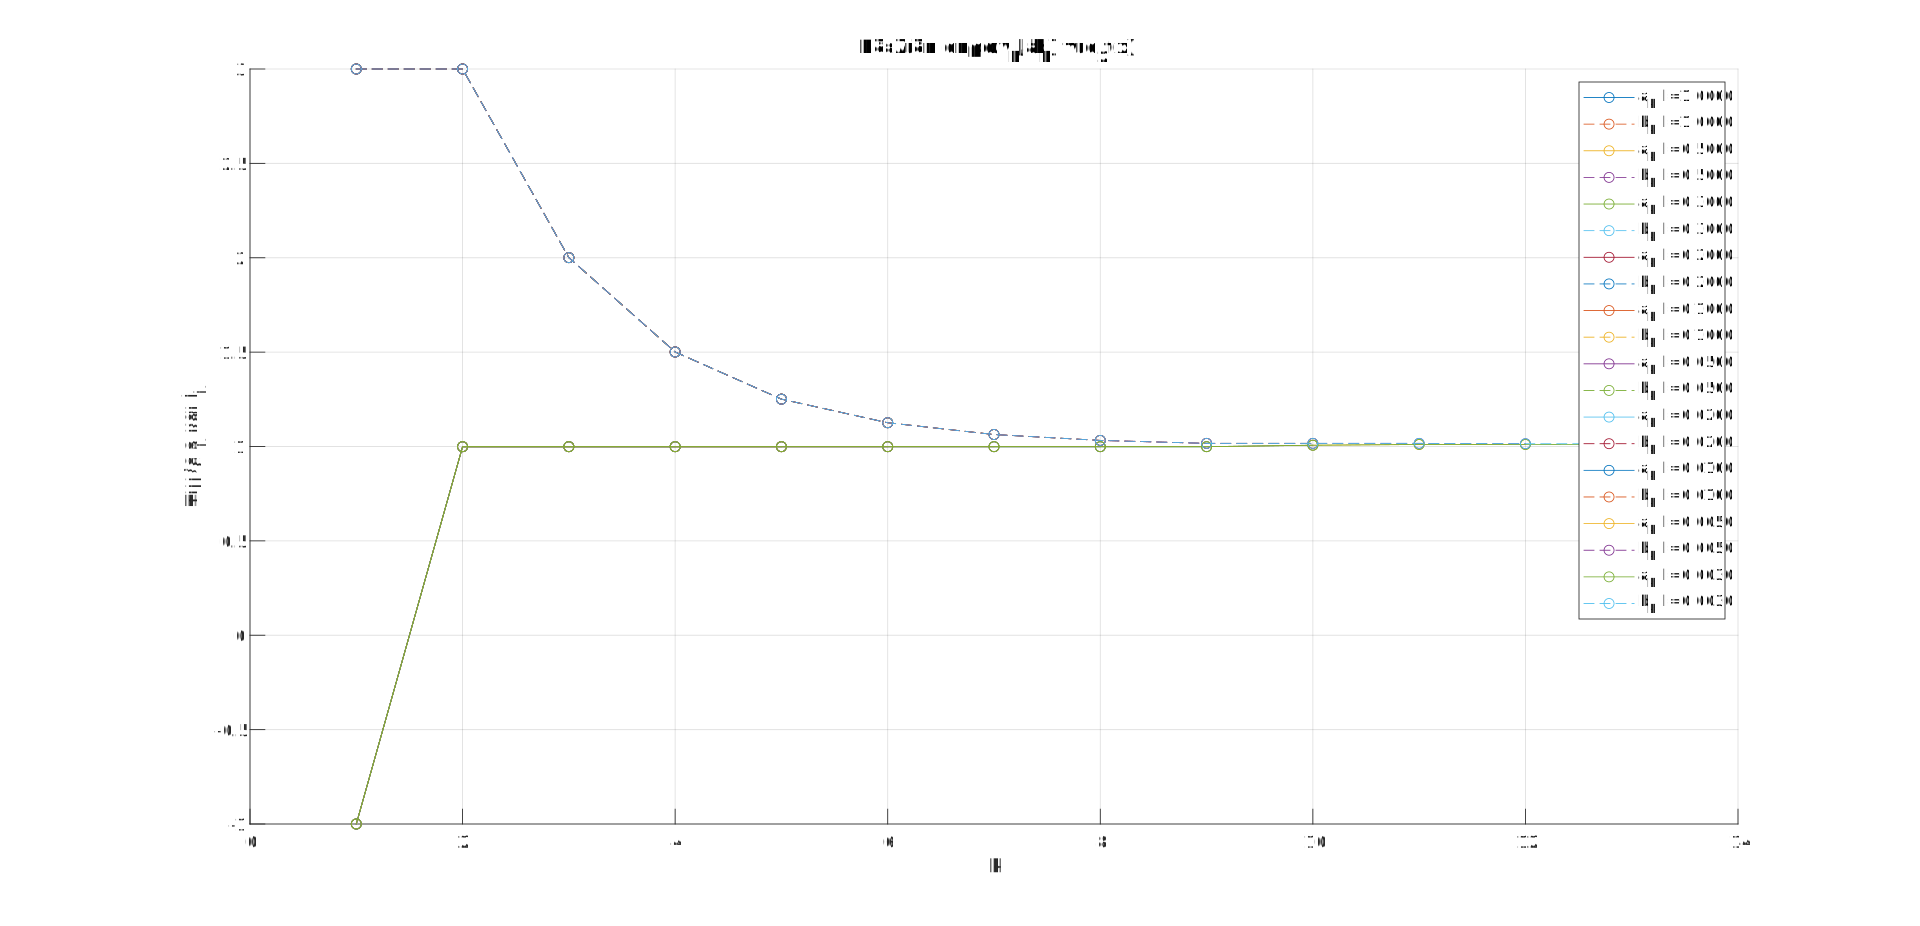
\includegraphics[width=0.7\textwidth]{dichotomous_interval_f2.png}
		\caption{Μεταβολή διαστήματος $[a_k, b_k]$ για την $f_2(x)$}
	\end{figure}
	
	\begin{figure}[H]
		\centering
		\includegraphics[width=0.7\textwidth]{dichotomous_interval_f3.png}
		\caption{Μεταβολή διαστήματος $[a_k, b_k]$ για την $f_3(x)$}
	\end{figure}
	
	\subsection{Μέθοδος Χρυσού Τομέα}
	
	\subsubsection{Μεταβολή υπολογισμών της $f$ συναρτήσει του $l$}
	Από τα γραφήματα παρατηρούμε ότι όσο μειώνεται η παράμετρος $l$, δηλαδή όσο αυξάνουμε την απαιτούμενη ακρίβεια της μεθόδου του χρυσού τομέα, τόσο αυξάνεται ο αριθμός των υπολογισμών της συνάρτησης. Η καμπύλη έχει τη χαρακτηριστική φθίνουσα μορφή: για μεγάλα $l$ η μέθοδος συγκλίνει πολύ γρήγορα, ενώ για μικρότερα $l$ απαιτούνται σημαντικά περισσότερα βήματα μέχρι να περιοριστεί το διάστημα αναζήτησης στο επιθυμητό εύρος. Το ενδιαφέρον είναι ότι η συμπεριφορά είναι σχεδόν ίδια και για τις τρεις συναρτήσεις, κάτι που επιβεβαιώνει ότι η μέθοδος του χρυσού τομέα έχει σταθερή και προβλέψιμη απόδοση, ανεξάρτητα από τη μορφή της μονοδιάστατης συνάρτησης. Συνολικά, τα αποτελέσματα δείχνουν ότι η μέθοδος είναι αξιόπιστη και αποδοτική, με το βασικό της “κόστος” να εμφανίζεται μόνο όταν απαιτούμε υψηλή ακρίβεια.
	Παρακάτω παραθέτω τα τρία γραφήμματα που δείχνουν πώς μεταβάλλεται ο αριθμός των υπολογισμών της $f$ όσο μεταβάλλουμε την σταθερά $l$.
	\begin{figure}[H]
		\centering
		\includegraphics[width=0.7\textwidth]{goldenSection_l_vs_fevals_f1.png}
		\caption{Μεταβολή υπολογισμών $f_1$ συναρτήσει του $l$}
	\end{figure}
	
	\begin{figure}[H]
		\centering
		\includegraphics[width=0.7\textwidth]{goldenSection_l_vs_fevals_f2.png}
		\caption{Μεταβολή υπολογισμών $f_2$ συναρτήσει του $l$}
	\end{figure}
	
	\begin{figure}[H]
		\centering
		\includegraphics[width=0.7\textwidth]{goldenSection_l_vs_fevals_f3.png}
		\caption{Μεταβολή υπολογισμών $f_3$ συναρτήσει του $l$}
	\end{figure}
	
	\subsubsection{Μεταβολή διαστήματος $[a_k,\, b_k]$ συναρτήσει του $k$}
	Από τα γραφήματα της εξέλιξης των άκρων $[a_k, b_k]$ για τις τρεις συναρτήσεις φαίνεται πολύ καθαρά ο τρόπος με τον οποίο η μέθοδος του χρυσού τομέα συρρικνώνει σταδιακά το αρχικό διάστημα προς το σημείο ελαχιστοποίησης. Για μεγάλα $l$ η σύγκλιση είναι ορατή ήδη από τα πρώτα 3–4 βήματα, με τα άκρα να μετακινούνται γρήγορα προς μια περιοχή κοινού σημείου. Όσο όμως μικραίνει το $l$, το διάστημα κλείνει πιο αργά και πιο “ήπια”, γεγονός που ταιριάζει απόλυτα με το ότι αυξάνεται ο αριθμός των απαιτούμενων υπολογισμών. Ένα ενδιαφέρον στοιχείο είναι ότι η γενική μορφή της σύγκλισης είναι σχεδόν ίδια και για τις τρεις συναρτήσεις: το διάστημα γίνεται μονότονα στενότερο και τελικά όλα τα ζεύγη $[a_k, b_k]$ συγκλίνουν σε μια συγκεκριμένη περιοχή όπου βρίσκεται το ελάχιστο. Αυτό ενισχύει την άποψη ότι η μέθοδος είναι σταθερή και προβλέψιμη, ανεξάρτητα από το ποια συνάρτηση έχουμε — απλώς για μεγαλύτερη ακρίβεια χρειάζεται πιο λεπτή σύγκλιση και άρα περισσότερα βήματα. Σε γενικές γραμμές, τα διαγράμματα δείχνουν ότι η μέθοδος του χρυσού τομέα επιτυγχάνει σταθερή, συστηματική σμίκρυνση του διαστήματος προς το ελάχιστο.
	Παρακάτω παραθέτω τα τρία γραφήμματα που δείχνουν πώς μεταβάλλεται το διάστημα $[a_k, b_k]$ συναρτήσει των επαναλήψεων $k$:
	\begin{figure}[H]
		\centering
		\includegraphics[width=0.7\textwidth]{goldenSection_intervals_f1.png}
		\caption{Μεταβολή διαστήματος $[a_k, b_k]$ για την $f_1(x)$}
	\end{figure}
	
	\begin{figure}[H]
		\centering
		\includegraphics[width=0.7\textwidth]{goldenSection_intervals_f2.png}
		\caption{Μεταβολή διαστήματος $[a_k, b_k]$ για την $f_2(x)$}
	\end{figure}
	
	\begin{figure}[H]
		\centering
		\includegraphics[width=0.7\textwidth]{goldenSection_intervals_f3.png}
		\caption{Μεταβολή διαστήματος $[a_k, b_k]$ για την $f_3(x)$}
	\end{figure}
	
	\subsection{Μέθοδος Fibonacci}
	
	\subsubsection{Μεταβολή υπολογισμών της $f$ συναρτήσει του $l$}
	Από τα γραφήματα της μεθόδου Fibonacci βλέπουμε ότι η συμπεριφορά της ως προς τον αριθμό αξιολογήσεων είναι παρόμοια με αυτή του χρυσού τομέα, αλλά λίγο πιο “πειθαρχημένη”. Καθώς η παράμετρος ακρίβειας $l$ μικραίνει, ο αριθμός των υπολογισμών αυξάνεται σταθερά και προβλέψιμα, ακολουθώντας την αύξηση του αντίστοιχου αριθμού Fibonacci που καθορίζει τα βήματα του αλγορίθμου. Το ενδιαφέρον είναι ότι οι καμπύλες για τις τρεις συναρτήσεις είναι ουσιαστικά ίδιες, κάτι που δείχνει πως η μέθοδος δεν επηρεάζεται ιδιαίτερα από το ίδιο το σχήμα της συνάρτησης. Σε σχέση με τον χρυσό τομέα, η Fibonacci καταλήγει συχνά να χρειάζεται ελαφρώς λιγότερες αξιολογήσεις για υψηλές απαιτήσεις ακρίβειας, κάτι που συμφωνεί και με τη θεωρία. Συνολικά, τα αποτελέσματα δείχνουν ότι η μέθοδος λειτουργεί αξιόπιστα και με σταθερό ρυθμό σύγκλισης, προσφέροντας μια σχεδόν βέλτιστη χρήση των αξιολογήσεων για κάθε επίπεδο ακρίβειας.
	Παρακάτω παραθέτω τα τρία γραφήμματα που δείχνουν πώς μεταβάλλεται ο αριθμός των υπολογισμών της $f$ όσο μεταβάλλουμε την σταθερά $l$.
	\begin{figure}[H]
		\centering
		\includegraphics[width=0.7\textwidth]{fibonacci_l_vs_fevals_f1.png}
		\caption{Μεταβολή υπολογισμών $f_1$ συναρτήσει του $l$}
	\end{figure}
	
	\begin{figure}[H]
		\centering
		\includegraphics[width=0.7\textwidth]{fibonacci_l_vs_fevals_f2.png}
		\caption{Μεταβολή υπολογισμών $f_2$ συναρτήσει του $l$}
	\end{figure}
	
	\begin{figure}[H]
		\centering
		\includegraphics[width=0.7\textwidth]{fibonacci_l_vs_fevals_f3.png}
		\caption{Μεταβολή υπολογισμών $f_3$ συναρτήσει του $l$}
	\end{figure}
	
	\subsubsection{Μεταβολή διαστήματος $[a_k,\, b_k]$ συναρτήσει του $k$}
	Στα διαγράμματα της εξέλιξης των άκρων $[a_k, b_k]$ για τη μέθοδο Fibonacci φαίνεται πολύ καθαρά ότι το διάστημα συρρικνώνεται με έναν εξαιρετικά σταθερό και “ρυθμισμένο” τρόπο. Σε αντίθεση με τον χρυσό τομέα, όπου η σύγκλιση είναι πιο ομοιόμορφη, εδώ τα άκρα αλλάζουν πιο “κοφτά” στα πρώτα βήματα επειδή καθορίζονται από τους αριθμούς Fibonacci, οι οποίοι επιβάλλουν μια συγκεκριμένη ακολουθία λόγων συρρίκνωσης. Όπως και να ’χει, το μοτίβο είναι το ίδιο σε όλες τις συναρτήσεις: το αριστερό και το δεξί άκρο κινούνται προς την περιοχή του ελαχίστου με τρόπο πλήρως συμμετρικό και τελικά τείνουν να επικαλύπτονται σε ένα πολύ στενό διάστημα. Για μικρότερα $l$ βλέπουμε ότι απαιτούνται περισσότερα βήματα μέχρι να σταθεροποιηθούν τα $[a_k, b_k]$, κάτι απόλυτα φυσιολογικό αφού η μέθοδος χρειάζεται μεγαλύτερη ακρίβεια. Το σημαντικό είναι ότι το σχήμα της σύγκλισης είναι σχεδόν ίδιο για όλες τις συναρτήσεις και όλα τα $l$: η Fibonacci παράγει μια προβλέψιμη, “βέλτιστα ελεγχόμενη” συρρίκνωση του διαστήματος, επιβεβαιώνοντας τη θεωρητική της ιδιότητα ότι χρησιμοποιεί με τον πιο αποδοτικό τρόπο τις διαθέσιμες αξιολογήσεις. Συνολικά, τα διαγράμματα δείχνουν ότι η μέθοδος όχι μόνο συγκλίνει ομαλά, αλλά και το κάνει ακριβώς με τον τρόπο που αναμένεται.
	Παρακάτω παραθέτω τα τρία γραφήμματα που δείχνουν πώς μεταβάλλεται το διάστημα $[a_k, b_k]$ συναρτήσει των επαναλήψεων $k$:
	\begin{figure}[H]
		\centering
		\includegraphics[width=0.7\textwidth]{fibonacci_intervals_f1.png}
		\caption{Μεταβολή διαστήματος $[a_k, b_k]$ για την $f_1(x)$}
	\end{figure}
	
	\begin{figure}[H]
		\centering
		\includegraphics[width=0.7\textwidth]{fibonacci_intervals_f2.png}
		\caption{Μεταβολή διαστήματος $[a_k, b_k]$ για την $f_2(x)$}
	\end{figure}
	
	\begin{figure}[H]
		\centering
		\includegraphics[width=0.7\textwidth]{fibonacci_intervals_f3.png}
		\caption{Μεταβολή διαστήματος $[a_k, b_k]$ για την $f_3(x)$}
	\end{figure}
	
	
	\subsection{Μέθοδος Διχοτόμου με Χρήση Παραγώγων}
	
	\subsubsection{Μεταβολή υπολογισμών της $f$ συναρτήσει του $l$}
	Στα διαγράμματα για τη μέθοδο διχοτόμησης με χρήση της παραγώγου φαίνεται ότι ο αριθμός των υπολογισμών της $f$ μειώνεται αρκετά γρήγορα όσο αυξάνεται το τελικό εύρος διαστήματος $l$. Η πτώση των αξιολογήσεων είναι πιο απότομη σε σχέση με τις μεθόδους Χρυσού Τομέα και Fibonacci, κάτι που βγάζει νόημα: η πληροφορία της παραγώγου επιτρέπει στο αλγόριθμο να εντοπίζει πολύ πιο «επιθετικά» προς ποια κατεύθυνση βρίσκεται το ελάχιστο και να απορρίπτει το μισό διάστημα σε κάθε βήμα. Έτσι, ακόμη και για αρκετά μικρές τιμές του $l$, ο αριθμός υπολογισμών παραμένει σχετικά χαμηλός και κινείται περίπου μεταξύ 5 και 11 για όλες τις συναρτήσεις. Παρατηρούμε, επίσης, ότι οι τρεις συναρτήσεις έχουν ουσιαστικά πανομοιότυπη συμπεριφορά, κάτι που υποδηλώνει πως το βασικό "κόστος" της μεθόδου εξαρτάται σχεδόν αποκλειστικά από το πόσο μικρό θέλουμε το τελικό διάστημα — όχι από τη μορφή της ίδιας της συνάρτησης. Συνολικά, τα διαγράμματα δείχνουν ότι η μέθοδος διχοτόμου με παράγωγο είναι ιδιαίτερα αποτελεσματική, παρέχοντας γρήγορη σύγκλιση και μικρό αριθμό υπολογισμών, το οποίο είναι αναμενόμενο, αφού αξιοποιεί ισχυρότερη πληροφορία (το πρόσημο της παραγώγου) σε κάθε βήμα.
	Παρακάτω παραθέτω τα τρία γραφήμματα που δείχνουν πώς μεταβάλλεται ο αριθμός των υπολογισμών της $f$ όσο μεταβάλλουμε την σταθερά $l$.
	\begin{figure}[H]
		\centering
		\includegraphics[width=0.7\textwidth]{dichotomousDerivative_l_vs_fevals_f1.png}
		\caption{Μεταβολή υπολογισμών $f_1$ συναρτήσει του $l$}
	\end{figure}
	
	\begin{figure}[H]
		\centering
		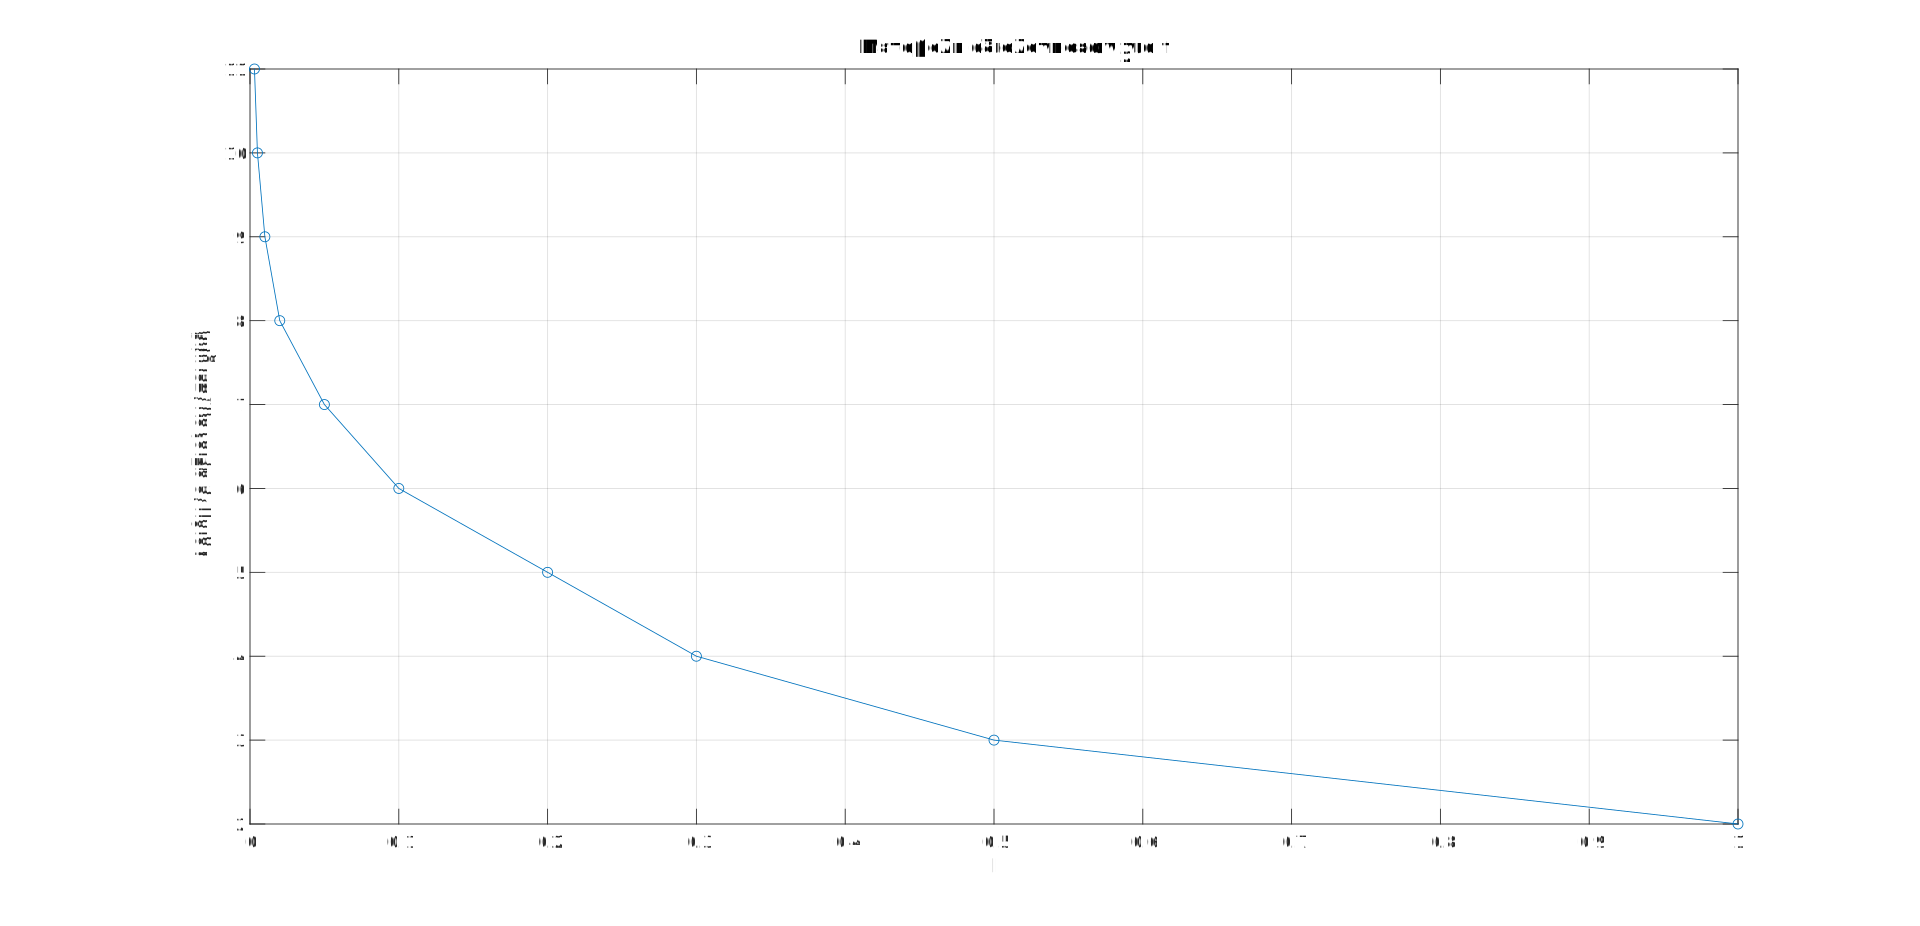
\includegraphics[width=0.7\textwidth]{dichotomousDerivative_l_vs_fevals_f2.png}
		\caption{Μεταβολή υπολογισμών $f_2$ συναρτήσει του $l$}
	\end{figure}
	
	\begin{figure}[H]
		\centering
		\includegraphics[width=0.7\textwidth]{dichotomousDerivative_l_vs_fevals_f3.png}
		\caption{Μεταβολή υπολογισμών $f_3$ συναρτήσει του $l$}
	\end{figure}
	
	\subsubsection{Μεταβολή διαστήματος $[a_k,\, b_k]$ συναρτήσει του $k$}
	Τα διαγράμματα δείχνουν ότι στη μέθοδο της διχοτόμου με παράγωγο το διάστημα $[a_k, b_k]$ συρρικνώνεται εξαιρετικά γρήγορα, επειδή σε κάθε βήμα ο αλγόριθμος συρρικνώνει το διάστημα με βάση το πρόσημο της παραγώγου. Το μοτίβο σύγκλισης είναι απόλυτα σταθερό και ίδιο για όλες τις συναρτήσεις: μετά από λίγα βήματα τα άκρα σχεδόν σταθεροποιούνται γύρω από το ελάχιστο, ενώ για μικρότερα $l$ απλώς συνεχίζεται η ίδια προβλέψιμη ημιτομή. Συνολικά, η μέθοδος εμφανίζεται πιο "κοφτή" και αποτελεσματική από τις προηγούμενες, αξιοποιώντας την πληροφορία της παραγώγου για να κατευθυνθεί πολύ γρήγορα στην περιοχή του ελαχίστου.
	Παρακάτω παραθέτω τα τρία γραφήμματα που δείχνουν πώς μεταβάλλεται το διάστημα $[a_k, b_k]$ συναρτήσει των επαναλήψεων $k$:
	\begin{figure}[H]
		\centering
		\includegraphics[width=0.7\textwidth]{dichotomousDerivative_interval_f1.png}
		\caption{Μεταβολή διαστήματος $[a_k, b_k]$ για την $f_1(x)$}
	\end{figure}
	
	\begin{figure}[H]
		\centering
		\includegraphics[width=0.7\textwidth]{dichotomousDerivative_interval_f2.png}
		\caption{Μεταβολή διαστήματος $[a_k, b_k]$ για την $f_2(x)$}
	\end{figure}
	
	\begin{figure}[H]
		\centering
		\includegraphics[width=0.7\textwidth]{dichotomousDerivative_interval_f3.png}
		\caption{Μεταβολή διαστήματος $[a_k, b_k]$ για την $f_3(x)$}
	\end{figure}
	
	\section{Συμπεράσματα}
	
	Συνολικά, τα πειραματικά αποτελέσματα δείχνουν με συνέπεια ότι και οι τέσσερις μέθοδοι συρρίκνωσης διαστήματος παρουσιάζουν προβλέψιμη και σταθερή συμπεριφορά, με τις διαφορές τους να προκύπτουν κυρίως από το πόση πληροφορία αξιοποιεί κάθε αλγόριθμος σε κάθε βήμα. Η κλασική μέθοδος της διχοτόμου είναι η πιο απλή και καθαρή ως προς τον ρυθμό σύγκλισης, αλλά απαιτεί τον μεγαλύτερο αριθμό αξιολογήσεων της συνάρτησης για υψηλή ακρίβεια. Η μέθοδος του χρυσού τομέα και η Fibonacci κάνουν πολύ πιο οικονομική χρήση των αξιολογήσεων, επιτυγχάνοντας πιο ομαλή συρρίκνωση του διαστήματος με σχεδόν πανομοιότυπη συμπεριφορά για όλες τις συναρτήσεις. Η Fibonacci υπερτερεί ελαφρώς όταν ζητείται υψηλή ακρίβεια, κάτι που συμφωνεί με τη θεωρητική της βελτιστοποίηση. Τέλος, η μέθοδος της διχοτόμου με χρήση παραγώγων είναι μακράν η πιο αποδοτική: αξιοποιεί το πρόσημο της παραγώγου ώστε να απορρίπτει ολόκληρο το μισό διάστημα σε κάθε επανάληψη, με αποτέλεσμα να χρειάζεται τον μικρότερο αριθμό αξιολογήσεων και να συγκλίνει με τον ταχύτερο ρυθμό. Σε όλες τις συναρτήσεις—και για όλα τα επίπεδα ακρίβειας—οι μέθοδοι παρουσιάζουν ουσιαστικά τα ίδια μοτίβα συμπεριφοράς, επιβεβαιώνοντας ότι η πολυπλοκότητά τους εξαρτάται κυρίως από το μήκος του τελικού διαστήματος και όχι από το σχήμα της ίδιας της συνάρτησης. Τα πειραματικά ευρήματα επιβεβαιώνουν τη θεωρητική ανάλυση, ότι η επιλογή μεθόδου επηρεάζει σημαντικά την υπολογιστική προσπάθεια, ειδικά όταν απαιτείται υψηλή ακρίβεια.
	
	\begin{table}[H]
		\centering
		\resizebox{\textwidth}{!}{
			\begin{tabular}{|c|c|c|c|c|}
				\hline
				\textbf{Μέθοδος} & \textbf{Ρυθμός Σύγκλισης} & \textbf{Αριθμός Αξιολογήσεων} & \textbf{Εξάρτηση από τη Συνάρτηση} & \textbf{Σχόλιο} \\
				\hline
				Διχοτόμος & Γεωμετρικός (μείωση κατά $1/2$) & Υψηλός για μικρό $l$ & Πολύ μικρή & Σταθερή αλλά όχι ιδιαίτερα οικονομική \\
				\hline
				Χρυσός Τομέας & Ομαλή μονομετρική συρρίκνωση & Μεσαίος & Πολύ μικρή & Προβλέψιμη και αξιόπιστη μέθοδος \\
				\hline
				Fibonacci & Βέλτιστη ως προς το πλήθος αξιολογήσεων & Ελαφρώς μικρότερος από Golden Section & Πολύ μικρή & Η πιο αποδοτική μέθοδος χωρίς παράγωγο \\
				\hline
				Διχοτόμος με Παράγωγο & Πολύ γρήγορη (κόβει το μισό διάστημα) & Χαμηλός – ο μικρότερος από όλες & Ανεξάρτητη από τη μορφή της συνάρτησης & Μακράν η πιο αποτελεσματική όταν υπάρχει παράγωγος \\
				\hline
			\end{tabular}
		}
		\caption{Συγκεντρωτική σύγκριση των τεσσάρων μεθόδων συρρίκνωσης διαστήματος.}
	\end{table}
	
\end{document}
